\chapter{A qubit: the two-level system}\label{ch:twolevel}

A qubit is any quantum system whose dynamics can be restricted to two states. Before treating the general case,
we solve the simplest example of the original notes and then explain where such Hamiltonians come from in nature.

\section{The simplest coupled two-level system}\label{sec:simplest}
Consider the Hamiltonian
\begin{equation}\label{eq:Hsimple}
  H=\begin{pmatrix}0&\hbar\omega/2\\ \hbar\omega/2&0\end{pmatrix}=\frac{\hbar\omega}2\sigma_x,
\end{equation}
which describes two states of equal energy (set to zero) coupled by a matrix element $\hbar\omega/2$.

\paragraph{Eigenvalues.} The characteristic equation is $\det(H-E)=E^2-(\hbar\omega/2)^2=0$, so $E_\pm=\pm\hbar\omega/2$.
\paragraph{Eigenvectors.} For $E_+=\hbar\omega/2$,
\begin{equation}
  \begin{pmatrix}0&\hbar\omega/2\\ \hbar\omega/2&0\end{pmatrix}\begin{pmatrix}\psi_1\\ \psi_2\end{pmatrix}
  =\frac{\hbar\omega}2\begin{pmatrix}\psi_1\\ \psi_2\end{pmatrix}
  \ \Longrightarrow\ \psi_2=\psi_1\ \Longrightarrow\ \psi_+=\frac1{\sqrt2}\begin{pmatrix}1\\1\end{pmatrix},
\end{equation}
and the eigenvector for $E_-=-\hbar\omega/2$ is orthogonal to it, $\psi_-=(1,-1)^T/\sqrt2$. Hence
\begin{equation}
  P=\frac1{\sqrt2}\begin{pmatrix}1&1\\1&-1\end{pmatrix}=P^{-1},
\end{equation}
(the Hadamard matrix, which is its own inverse).
\paragraph{Evolution operator.} By \cref{eq:Udiag},
\begin{equation}\label{eq:Usimple}
  U(t)=P\begin{pmatrix}\e^{-\ii\omega t/2}&0\\0&\e^{\ii\omega t/2}\end{pmatrix}P^{-1}
  =\begin{pmatrix}\cos\frac{\omega t}2&-\ii\sin\frac{\omega t}2\\-\ii\sin\frac{\omega t}2&\cos\frac{\omega t}2\end{pmatrix}
  =\cos\tfrac{\omega t}2\,I-\ii\sin\tfrac{\omega t}2\,\sigma_x .
\end{equation}
Let us check the matrix product explicitly for the $(1,1)$ element: $\frac12(\e^{-\ii\omega t/2}+\e^{\ii\omega t/2})=\cos\frac{\omega t}2$;
for the $(1,2)$ element: $\frac12(\e^{-\ii\omega t/2}-\e^{\ii\omega t/2})=-\ii\sin\frac{\omega t}2$. The last form also follows directly
from \cref{prop:involution} since $\sigma_x^2=I$.

\paragraph{Dynamics.} For $\psi(0)=(1,0)^T$,
\begin{equation}
  \psi(t)=\begin{pmatrix}\cos\frac{\omega t}2\\-\ii\sin\frac{\omega t}2\end{pmatrix},\qquad
  P_1(t)=\abs{\begin{pmatrix}1&0\end{pmatrix}\psi(t)}^2=\cos^2\frac{\omega t}2=\frac{1+\cos\omega t}2.
\end{equation}
The system oscillates between the two states at the frequency $\omega=(E_+-E_-)/\hbar$, the Bohr frequency of the
two eigenstates (\cref{fig:rabi}). The probability is periodic with period $2\pi/\omega$, while the state vector itself has period $4\pi/\omega$:
$U(2\pi/\omega)=-I$. This sign is a global phase and is not observable here, but it becomes observable when the two-level system is
part of an interferometer (the famous $4\pi$ periodicity of spinors, observed with neutrons in 1975).

\begin{figure}[h]\centering
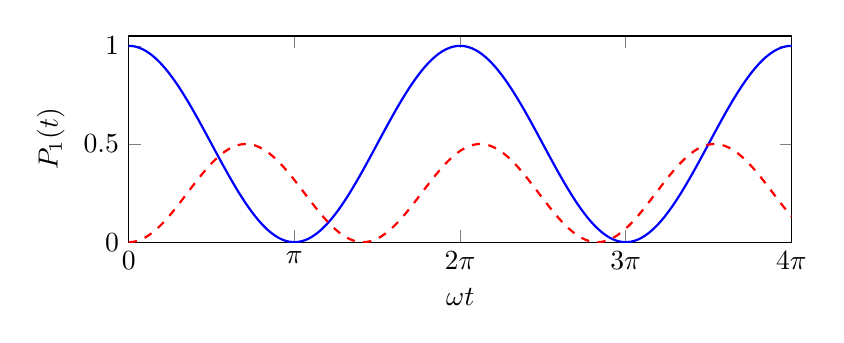
\begin{tikzpicture}
\begin{axis}[width=10cm,height=4.2cm,xlabel={$\omega t$},ylabel={$P_1(t)$},xmin=0,xmax=12.57,ymin=0,ymax=1.05,
  xtick={0,3.1416,6.2832,9.4248,12.566},xticklabels={$0$,$\pi$,$2\pi$,$3\pi$,$4\pi$},ytick={0,0.5,1}]
\addplot[blue,thick,domain=0:12.57,samples=200]{cos(deg(x/2))^2};
\addplot[red,dashed,thick,domain=0:12.57,samples=200]{0.5*sin(deg(sqrt(2)*x/2))^2};
\end{axis}\end{tikzpicture}
\caption{Solid: resonant oscillation $P_1=\cos^2(\omega t/2)$. Dashed: probability to reach the other state for a detuned
system with $\Delta=\Omega$, \cref{eq:rabiformula}: the oscillation is faster and incomplete.}\label{fig:rabi}
\end{figure}

\paragraph{A quantum gate.} At $\omega t=\pi$, $U=-\ii\sigma_x$: up to the global phase $-\ii$, the evolution has implemented the NOT gate
$X=\sigma_x$, exchanging $\ket0$ and $\ket1$. A ``$\pi$-pulse'' is a NOT gate. At $\omega t=\pi/2$ we get
$U=(I-\ii\sigma_x)/\sqrt2$, which transforms $\ket0$ into the equal superposition $(\ket0-\ii\ket1)/\sqrt2$: a ``$\pi/2$-pulse'' creates
superpositions. All single-qubit gates are realised in this way, by letting the qubit evolve under a chosen Hamiltonian for a chosen
time. In the Bloch-sphere language of \cref{ch:bloch}, $U(t)$ is a rotation of the pseudospin about the $x$ axis by the angle $\omega t$,
which brings $\vec S=S_z\vec e_z$ to $-S_z\vec e_z$ at $\omega t=\pi$.

\section{Physical origin of two-level Hamiltonians}
Where do Hamiltonians like \cref{eq:Hsimple} come from? Real systems have infinitely many levels. A two-level description is an
\emph{effective model}, valid when only two levels are involved in the dynamics. Here are three fundamental examples.

\subsection{A particle in a double well: the ammonia molecule}\label{sec:doublewell}
\begin{origin}[: tunnelling in a double well]
Consider a particle in a symmetric double-well potential $V(x)$, with two minima at $\pm a$ separated by a barrier. If the barrier
is high, the low-energy states are well described by the two states $\ket L$ and $\ket R$ localized in the left and right wells
(for example the ground states of each well considered alone, of energy $E_0$). We look for eigenstates in the form
$\ket\psi=c_L\ket L+c_R\ket R$ (a variational, or ``tight-binding'', ansatz). Projecting $H\ket\psi=E\ket\psi$ onto $\bra L$ and $\bra R$,
and neglecting the small overlap $\braket LR$,
\begin{equation}
  H_{\rm eff}=\begin{pmatrix}\mel LHL&\mel LHR\\ \mel RHL&\mel RHR\end{pmatrix}=\begin{pmatrix}E_0&-A\\-A&E_0\end{pmatrix}.
\end{equation}
The diagonal elements are equal by symmetry. The off-diagonal element $-A$ is the \emph{tunnelling amplitude}: it is non-zero because the
wave function of $\ket L$ has an exponentially small tail under the barrier and in the right well. A WKB estimate gives
$A\simeq\frac{\hbar\omega_0}{\pi}\exp\left(-\frac1\hbar\int_{-b}^{b}\sqrt{2m(V(x)-E_0)}\,\dd x\right)$, where $\omega_0$ is the oscillation
frequency in one well and $\pm b$ are the classical turning points: the tunnelling is exponentially sensitive to the height and width of the barrier.

Dropping $E_0$ (a global phase), $H_{\rm eff}=-A\sigma_x$, i.e.\ \cref{eq:Hsimple} with $\hbar\omega/2=-A$. The eigenstates are the
symmetric and antisymmetric combinations $(\ket L\pm\ket R)/\sqrt2$, split by $2A$. A particle initially in the left well oscillates
between the two wells at the frequency $2A/\hbar$.

\emph{The ammonia molecule} NH$_3$ is the textbook example (Feynman Lectures, vol.~III, chap.~8--9). The nitrogen atom can be above or
below the plane of the three hydrogen atoms: these are $\ket L$ and $\ket R$. Tunnelling of the nitrogen through the plane splits the
ground state into two levels separated by $2A/h\approx23.87$\,GHz. This transition was used in the first maser (Townes, 1954). Feynman,
Vernon and Hellwarth introduced the geometrical (pseudospin) representation of the next chapter precisely to describe masers \cite{FVH1957}.
\end{origin}

The same model describes an electron in a double quantum dot (charge qubit), a Cooper pair box (\cref{ch:implementations}),
a flux qubit (clockwise vs anticlockwise current), or a photon in two coupled waveguides (directional coupler).

\subsection{A spin 1/2 in a magnetic field}\label{sec:spin}
\begin{origin}[: the Zeeman Hamiltonian]
A particle with spin $\vec S=\frac\hbar2\vec\sigma$ has a magnetic moment $\vec\mu=\gamma\vec S$, where $\gamma$ is the gyromagnetic ratio
($\gamma=-g_e e/2m_e$ with $g_e\approx2$ for the electron, $\gamma/2\pi=42.58$\,MHz/T for the proton). As for a classical magnetic dipole, its
energy in a magnetic field $\vec B$ is
\begin{equation}
  H=-\vec\mu\cdot\vec B=-\frac{\hbar\gamma}2\,\vec B\cdot\vec\sigma.
\end{equation}
This is the most general traceless $2\times2$ Hermitian matrix (\cref{sec:pauli}): any two-level Hamiltonian is formally that of a spin in an
effective magnetic field. A field along $z$ splits the levels by $\hbar\gamma B$ (Zeeman effect); a field along $x$ couples them as in
\cref{eq:Hsimple}. The spin precesses about $\vec B$ at the Larmor frequency $\omega_L=\gamma B$. Nuclear magnetic resonance
(\cref{sec:nmr}) and electron spin qubits in quantum dots use exactly this Hamiltonian.
\end{origin}

\subsection{An atom driven by a laser: Rabi oscillations}\label{sec:rabi}
\begin{origin}[: the electric-dipole Hamiltonian and the rotating-wave approximation]
Consider two levels $\ket g=\ket0$ and $\ket e=\ket1$ of an atom, with energy difference $\hbar\omega_0$, and an electric field
$\vec E(t)=\vec E_0\cos\omega t$ of a laser. Since the wavelength (${\sim}500$\,nm) is much larger than the atom (${\sim}0.1$\,nm), the field is
uniform over the atom (\emph{dipole approximation}) and the coupling is $V=-\hat{\vec d}\cdot\vec E(t)$, where $\hat{\vec d}=-e\hat{\vec r}$ is the
electric dipole operator. (It is obtained from the minimal-coupling Hamiltonian $(\vec p+e\vec A)^2/2m$ by a gauge transformation, the
Göppert-Mayer transformation.) For atomic states of well-defined parity, $\mel g{\vec r}g=\mel e{\vec r}e=0$, so only the off-diagonal elements
$\vec d_{eg}=\mel e{\hat{\vec d}}g$ survive. Choosing the phases of the states so that $\vec d_{eg}\cdot\vec E_0$ is real, and setting
$\hbar\Omega=-\vec d_{eg}\cdot\vec E_0$,
\begin{equation}\label{eq:Hdriven}
  H(t)=-\frac{\hbar\omega_0}2Z+\hbar\Omega\cos(\omega t)\,X,
\end{equation}
where $Z=\proj0-\proj1$, so that $\ket0=\ket g$ has energy $-\hbar\omega_0/2$.

This Hamiltonian is time dependent. We go to a frame rotating at the laser frequency, $\ket{\tilde\psi}=R(t)\ket\psi$ with
$R=\e^{-\ii\omega tZ/2}$. By \cref{eq:frame}, $\ii\hbar\dot RR^\dagger=\frac{\hbar\omega}2Z$, and
$RXR^\dagger=\cos(\omega t)X+\sin(\omega t)Y$ (\cref{prop:bch}). Hence
\begin{equation}
  \tilde H=-\frac{\hbar\Delta}2Z+\frac{\hbar\Omega}2\Big[X\big(1+\cos2\omega t\big)+Y\sin2\omega t\Big],\qquad\Delta=\omega_0-\omega.
\end{equation}
Near resonance, $|\Delta|,\Omega\ll\omega$, the terms oscillating at $2\omega$ average to zero over the slow dynamics, which takes place on the
time scale $1/\Omega$. Neglecting them is the \emph{rotating-wave approximation} (RWA), and gives a time-independent Hamiltonian:
\begin{equation}\label{eq:HRWA}
  \tilde H_{\rm RWA}=\frac\hbar2\left(-\Delta\,Z+\Omega\,X\right).
\end{equation}
The neglected terms give a small shift of the resonance, the Bloch--Siegert shift $\Omega^2/4\omega$.
\end{origin}

\paragraph{Rabi formula.} $\tilde H_{\rm RWA}=\frac{\hbar\Omega_R}2\,\vec n\cdot\vec\sigma$ with the \emph{generalized Rabi frequency}
$\Omega_R=\sqrt{\Omega^2+\Delta^2}$ and the unit vector $\vec n=(\Omega,0,-\Delta)/\Omega_R$. By \cref{prop:involution},
\begin{equation}
  \tilde U(t)=\cos\frac{\Omega_Rt}2\,I-\ii\sin\frac{\Omega_Rt}2\,\vec n\cdot\vec\sigma,
\end{equation}
and the probability to find the atom excited, starting from $\ket g$, is $|\mel1{\tilde U}0|^2$ (the frame change $R$ only adds phases):
\begin{equation}\label{eq:rabiformula}
  P_e(t)=\frac{\Omega^2}{\Omega^2+\Delta^2}\,\sin^2\frac{\sqrt{\Omega^2+\Delta^2}\,t}2.
\end{equation}
This is Rabi's formula (I.~I.~Rabi, 1937, for spins in magnetic fields). At resonance ($\Delta=0$) the transfer is complete; off
resonance it is faster and incomplete (\cref{fig:rabi}). The Lorentzian prefactor $\Omega^2/(\Omega^2+\Delta^2)$ is the line shape of
the transition: it has a width $\sim\Omega$ (power broadening). For a qubit, the lesson is that gates are made by \emph{resonant pulses}:
the frequency $\omega$ selects which transition is driven, and the pulse area $\Omega t$ selects the rotation angle. The phase of the
drive ($\cos\omega t$ vs $\sin\omega t$) selects the rotation axis ($X$ or $Y$), as you can check by repeating the derivation with
$\sin\omega t$.

\begin{keypoint}
All single-qubit gates in the laboratory are rotations generated by Hamiltonians of the form \cref{eq:HRWA}. The original example
\cref{eq:Hsimple} is the resonant case $\Delta=0$, $\Omega=\omega$.
\end{keypoint}

\section{Exercises}
\begin{exercise}
Derive \cref{eq:rabiformula} directly by solving the coupled equations for the amplitudes $c_g(t)$, $c_e(t)$ in the rotating frame.
\end{exercise}
\begin{exercise}
For the ammonia molecule, estimate $A$ in eV from $2A/h=23.87$\,GHz. Compare with the thermal energy at room temperature. What fraction
of molecules is in the upper state at $300$\,K? (Answer: $A\approx4.9\times10^{-5}$\,eV, nearly one half.) Why does this make a maser
possible only after a state selection (Townes used an electrostatic focuser)?
\end{exercise}
\begin{exercise}
Repeat the RWA derivation with the drive $\hbar\Omega\sin(\omega t+\phi)X$. Show that the effective Hamiltonian is
$\frac\hbar2(-\Delta Z+\Omega(\sin\phi\,X+\cos\phi\,Y))$, so that the phase of the microwave or laser selects the rotation axis in the $xy$ plane.
\end{exercise}
